
% Experement data + calcs goes here %

\section{Ход работы}
\subsection{Характеристики шариков}
Измерил характеристики шариков и типовые расстояния - данные сошлись с теорией и при различных способах измерения (см листик с данными).

\subsection{Измерение горизонтальной составляющей магнитного поля земли}

Зависимость периода от количества шариков представлена на рисунке 4. Видно, что эта зависимость линейна, что соглауется с теорией. Данные см на листике с данными.

\begin{center}

    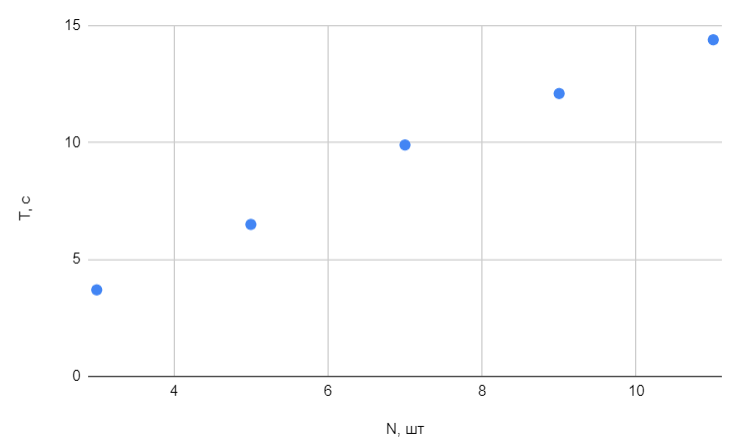
\includegraphics[scale=0.9]{picks/121-graph1.png} \\
    \textit{Рис. 4. T(N)}

\end{center}

\noindentЗначение горизонтальной составляющей магнитного поля (через период колебаний): \\
\mth{B_n = 24,22 \pm 0,34} мкТл.

\newpage

\subsection{Измерение вертикальной составляющей магнитного поля земли}

Зависимость уравновешивающей массы от плеча представлена на рисунке 5. Видно, что она имеет вид \mth{\frac{1}{x}}, что согласуется с теорией. Однако, следует отметить, что данный метод измерения весьма не точен. Поэтому, схождения с теорией ожидать не следует.

\begin{center}

    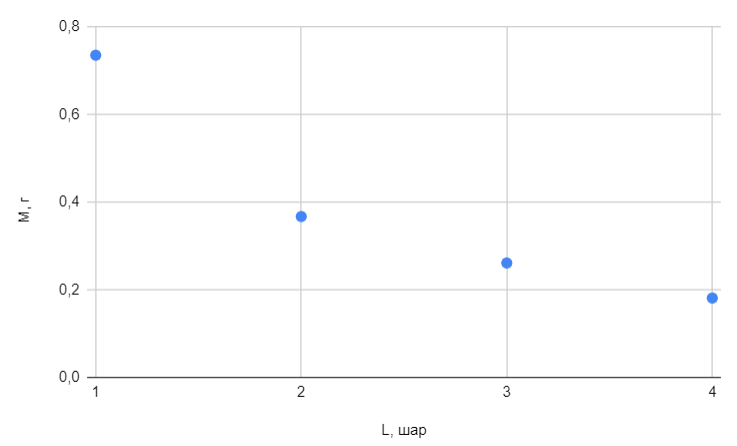
\includegraphics[scale=0.9]{picks/121-graph2.png} \\
    \textit{Рис. 5. M(L)}

\end{center}

\noindentЗначение вертикальной составляющей магнитного поля (через уравновешиваюущую массу):\\
\mth{B_v = 33,71 \pm 0,84} мкТл.

\noindentТогда суммарное значение для магнитного поля земли: \mth{B = 41,7 \pm 0,91} мкТл.

\section{Вывод}

В ходе данной работы были расчитаны фундаментальные характеристики неодиомовых магнитов. Данные характеристики близки к реальным значениям. Также были произведены ойценки для значений вертикальной и горизонтальной составляющих магнитного поля земли. Для горизонтальной составляющей оценка оказалась весьма точна.